%!TEX TS-program = xelatex
%!TEX encoding = UTF-8 Unicode

\documentclass[12pt, a4paper]{scrartcl}

%% Page Layout
\usepackage[margin=1in]{geometry}

\usepackage{euler} % math font package needs to be loaded before others
\usepackage{xunicode,xltxtra, polyglossia}
\setdefaultlanguage[variant=american]{english}

%% fonts, symbols, text
	%%% fonts
	\usepackage{fontspec} %(include if mathspec is not loaded)
	\defaultfontfeatures{Mapping=tex-text, Ligatures=TeX}
	%%% text decoration
	\usepackage[normalem]{ulem} % sout
	%%% semantics symbols
	\usepackage{stmaryrd}
	\usepackage{amsmath,amssymb}
	\newcommand{\transl}{\rightsquigarrow \ensuremath}
	%%% other symbols
	\usepackage{pifont}% http://ctan.org/pkg/pifont
	\newcommand{\cmark}{\ding{51}}%
	\newcommand{\xmark}{\ding{55}}%

%% layout
%%% page layout
\usepackage{multicol}


%% bibliography
\usepackage[round]{natbib}
\newcommand{\posscite}[1]{\citeauthor{#1}'s (\citeyear{#1})}

%% figures, examples, diagrams
%%% examples
\usepackage{linguex}
\renewcommand{\firstrefdash}{}
%%% tables 
\usepackage{booktabs}
%%% figures
\usepackage{graphics}


%% decoration and features
%%% colors
\usepackage[dvipsnames]{xcolor}

%% bibliography
\renewcommand*{\refname}{\normalsize\textbf{References}\\ \vspace{-.5\baselineskip}}

%% fonts
\setmainfont[Scale=MatchLowercase,Mapping=tex-text,SmallCapsFont={TeX Gyre Termes}, SmallCapsFeatures={Letters=SmallCaps}]{Times New Roman}
\setsansfont[Scale=MatchLowercase,Mapping=tex-text]{Times New Roman}

\usepackage{setspace}
\begin{document}

\bibliographystyle{plainnat}
% \enablehyphenation
% \vspace{-2em}
% \maketitle
\textcolor{white}{.} \vspace{-2.9\baselineskip} \\
\begin{center}
	\textbf{\large%\thetitle
		A diverse family (of sentences)\\ Projectivity differs across embedding operators---but not like you think}
\end{center}

\vspace{-.5\baselineskip}
\noindent We present experimental evidence that the projectivity of attitude complements varies across different entailment-cancelling operators, and that this effect of entailment-cancelling operator differs between various attitude verb triggers. However, our findings about the interaction of operator and trigger do not support \posscite{karttunen_observations_1971} classification of factive vs. semi-factive verbs.

\vspace{-\baselineskip}
\paragraph{Projection across various entailment-cancelling operators.}
	Certain attitude ascriptions come with an inference to the truth of their complement, even if embedded under entailment-cancelling operators (illustrated for \emph{\lq discover\rq} in \ref{ex:family}), in which case this inference is said to \emph{project}, (e.g. \citealp{karttunen_observations_1971}).

	\vspace{-.25\baselineskip}
	\ex. \label{ex:family}
		\a. Polar Questions: \hfill
			\emph{\lq Did Cole discover that Julian dances Salsa?\rq}
		\b. Negation: \hfill
			\emph{\lq Cole didn't discover that Julian dances Salsa.\rq}
		\b. Modals: \hfill
			\emph{\lq Perhaps Cole discovered that Julian dances Salsa.\rq}
		\b. Conditionals: \hfill
			\emph{\lq If Cole discovered that Julian dances Salsa, Logan will be joyful.\rq}
		\z.
	\z.

	\vspace{-.25\baselineskip}
	Previous work on projection showed that it is not a categorial property of lexical triggers \citep{tonhauser_how_2018}, but a gradient one affected by various contextual factors \citep{simons_what_2010,de_marneffe_did_2012,beaver_questions_2017,degen_prior_2021}. In light of this, we expect that the hetergeneous entailment-cancelling operators in \ref{ex:family} affect projection differentially.

	Generalizations to this effect were suggested by \citet{karttunen_observations_1971}, who distinguishes between \emph{factive} verbs (\emph{regret, forget, resent}) and \emph{semi-factive} verbs (\emph{discover, realize, see, find out, notice}), suggesting that factives always project, while semi-factives always project across negation, but not always in polar questions or conditionals. SMITH study, Djärv on conitive/emotive difference.
	We experimentally test these generaliztions in a study addressing the questions: \textbf{(i)} Is the projection of content affected by differences in entailment-canceling environments? \textbf{(ii)} Do these effects vary for different verbs (and in what way)?

\vspace{-\baselineskip}
\paragraph{Experimental investigation.} % (fold)
	% Using an experimental task designed to assess speaker commitment to the complement clause, we find that the choice of entailment-cancelling operator affects projection, and that there are differences between triggers in their interaction with embedding operators. 

	To investigate differences in projection behavior across various en- tailment-cancelling operators as in \ref{ex:family}, and between various types of attitude verbs, we used a response task which elicitied participant judgments about how strongly they thought a speaker would be committed towards the embedded clause. We presented sentences like in \ref{ex:family} as asserted by a named speaker (on screen as e.g. “\textbf{Daniel:} \emph{\lq Did Cole\dots?\rq}”). Participants were then asked to provide a judgment in response to a prompt like: \emph{“Is Daniel certain that Julian dances Salsa?”}), by moving a slider on a scale from \lq no\rq\ (coded as \texttt{0}), to \lq yes\rq\ (coded as \texttt{1}). 

% paragraph experiment (end)

\paragraph{Design and Expectations.} % (fold)
	\ex. 20 clause-embedding predicates 
		\a. canonically factive: {\em be annoyed, discover, know, reveal, see}
		\b. nonfactive:
			\a. nonveridical nonfactive: {\em pretend, suggest, say, think}
			\b. veridical nonfactive: {\em be right, demonstrate}
			\z.
		\b. optionally factive: {\em acknowledge, admit, announce, confess, confirm, establish, hear, inform, prove}
		\z.
	\z.

	\begin{itemize}
		\item Expectations based on Karttunen:
		\begin{itemize}
			\item no variation for factive verbs
			\item semi-factives (like \emph{discover}) should project more strongly across negation than questions
		\end{itemize}

		\item expectations based on Djärv:
		\begin{itemize}
			\item emotive predicates (like \emph{be annoyed}) behave like Karttunen's factives
			\item cognitive predicates (like \emph{discover, see\dots}) behave like Karttunen's semi-factives
		\end{itemize}
	\end{itemize}

% paragraph design_and_expectations_ (end)

\paragraph{Method.} % (fold)
	\dots
% paragraph method (end)

\paragraph{Results and Analysis.} % (fold)
	\begin{itemize}
		\item pooled data across experiments
	\end{itemize}

	\textbf{Figure \ref{fig:figure1}} shows the mean certainty-ratings by operator and predicate, and 95\% bootstrapped confidence intervals.

	\begin{figure}[h]
		\centering
		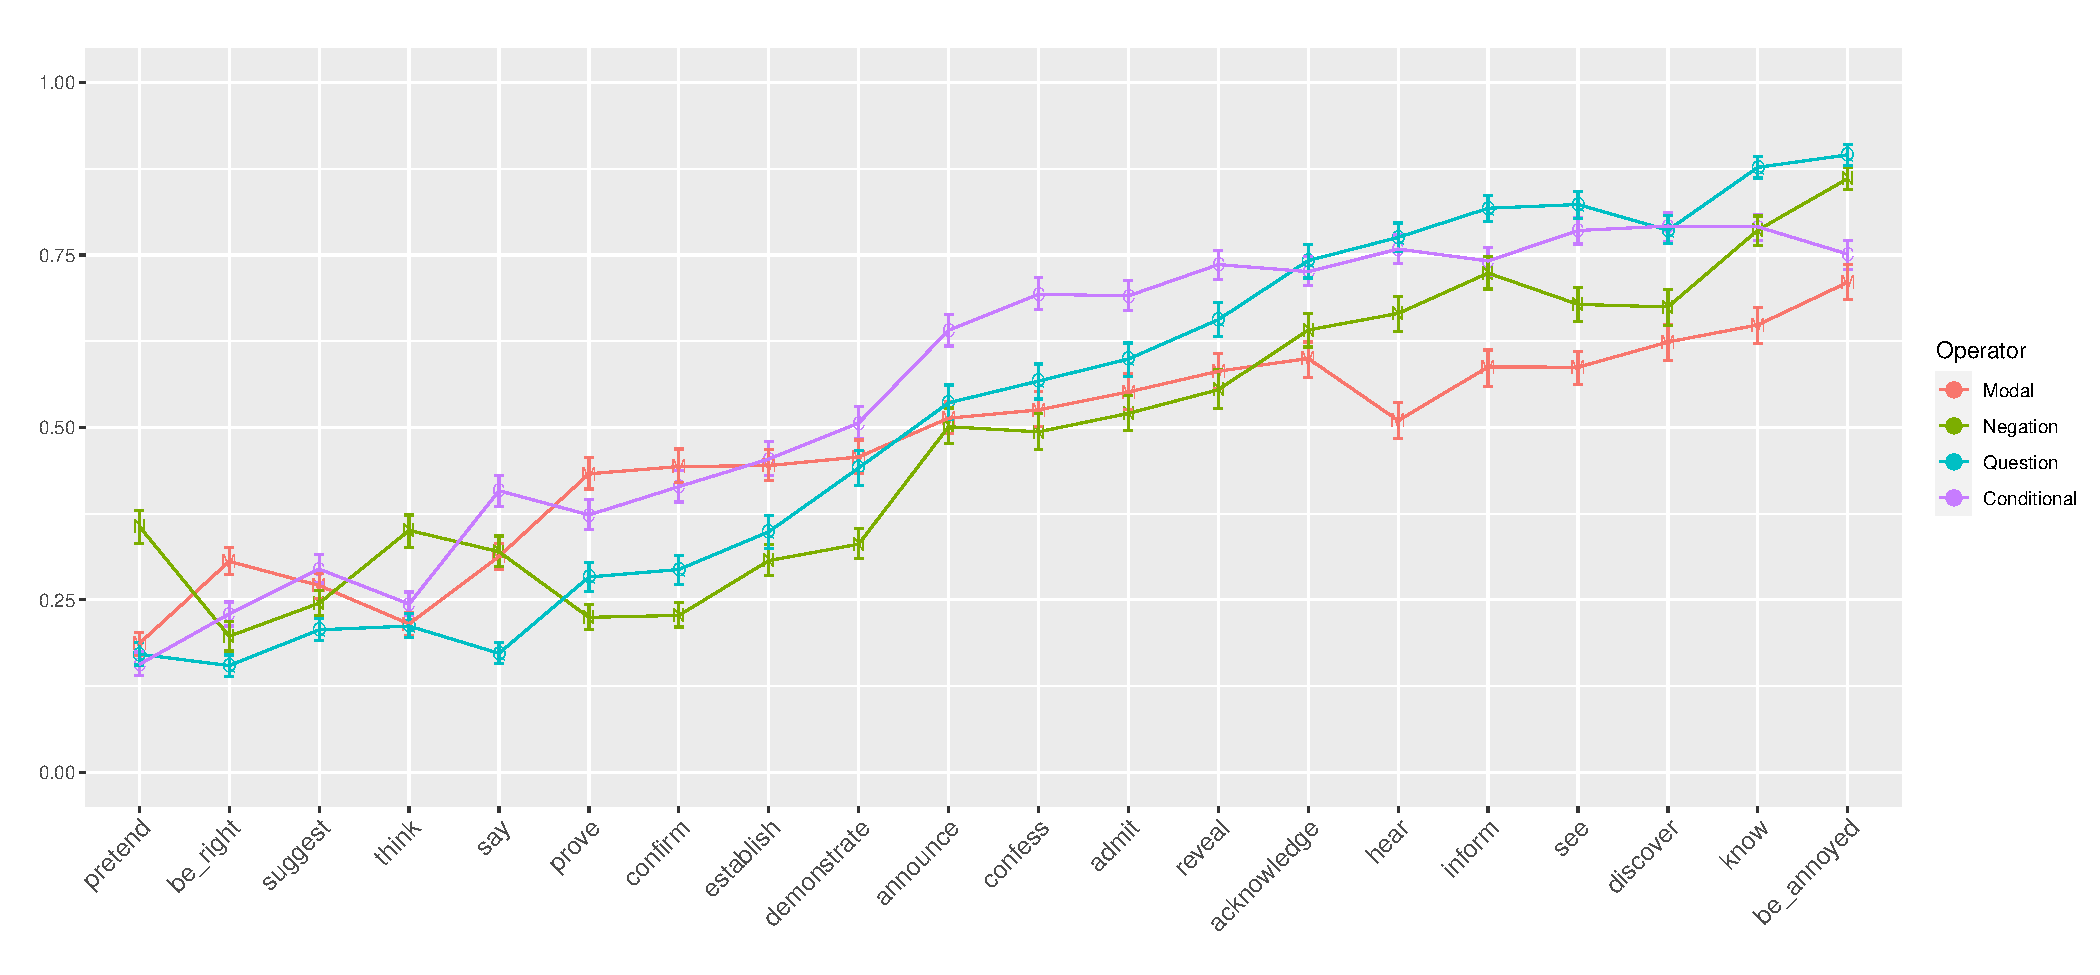
\includegraphics[width=\textwidth]{graphs/proj-by-both.pdf}
		\caption{Mean certainty ratings by operator and predicate}
		\label{fig:figure1}
	\end{figure}

	\begin{itemize}
		\item The embedding operator affects projection (main effect of embedding operator)
		\item This effect differs by verb (interaction effects of operator/verb)
	\end{itemize}
% paragraph method (end)

\paragraph{Discussion and Conclusion.} % (fold)
	\dots
% paragraph method (end)

\pagebreak
\bibliography{projective-content.bib}

\end{document}